\documentclass{article}
\usepackage{graphicx}

\begin{document}

\title{Team Meeting 2 Summary}
\author{Christian Plourde 26572499\\*
		Ayush Kharade 40042388\\*
		Daniel Vellucci 27416288\\*
		Samer Yazbeck 40049573\\*
		Luciano Porchet 40048537
		}
\date{September 25th, 2019}

\maketitle

\newpage

\section{Meeting Duration}
75 Minutes

\section{Notes}
\subsection{Game Details}
\begin{description}
\item 3D characters, Platformer in a 2D view
\item Platformer
\item Singleplayer
\item Similar to Trine or This War of Mine
\item Genre: Action / Adventure platformer
\end{description}

\subsection{Story}
\begin{description}
\item Main character is Mistborn (NAME: YORA)
\item Main character loses crew member at sea, traumatic experience occurs, he snaps gets access to his powers
\item Makes it to abandoned village
\item Hears thumping sound drawing him to the Well of Ascension
\item Starts moving toward the thumping
\item When character makes it there he is confronted by Ruin - boss fight
\end{description}

\subsection{Enemies}
\begin{description}
\item Coinshots(ranged?)
\item Regular minions (people under Ruin’s Control)
\item Boss (Ruin)
\end{description}

\subsection{Mistborn Mechanics}
\begin{description}
\item Burning metals (magic system called allomancy)
\item Iron - pull metal objects toward you
\item Steel - push metal objects away from you
\item Pewter - Makes user stronger, more agile, increases endurance and healing
\item Collect metals from the environment (pots, rocks, chests)
\item Small puzzles with iron and steel (Steppable platforms that open something like doors), Levers
\item Ruin can change words (give fake hints to the player) player gambles if it is worth going there (could have traps or very powerful enemies in these areas)
\item Death takes you a checkpoint
\item Climbable walls
\item Traps (pit with spikes)
\item If you run out of metals, go back to past place where you got the resources before (once you have run out it instantly restocks)
\item Objects can drop when pulled can be used in puzzles or fighting
\item Progression issue - if someone runs out of metals, how can they complete the level.
Need to figure out what happens if player runs out of metals, (restocks supplies).
\end{description}

\subsection{Mistborn Setting}
\begin{description}
\item Black world, falling ash, red sun
\item Misty Environment
\end{description}

\subsection{Combat}
\begin{description}
\item Steel, iron fighting moving metal objects
\item Melee only available when you burn pewter
\end{description}

\subsection{Enemy Mechanics}
\begin{description}
\item Only attack if close enough, move towards you until it is close enough
\item Chase you to the end of the room then go back
\end{description}

\subsection{Sound Effects}
\begin{description}
\item Sound when player walks
\end{description}

\subsection{Supporting Art}
  \begin{figure}[!htb]
    \center{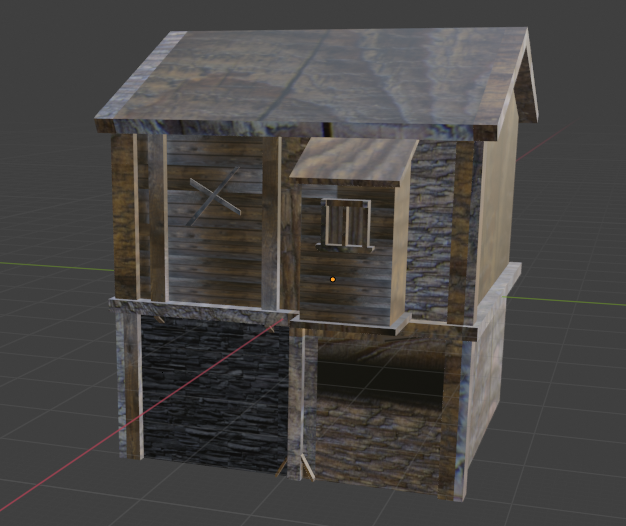
\includegraphics[width=5cm, height=5cm]
    {skaa_building_1.png}}
  \end{figure}

  \begin{figure}[!htb]
    \center{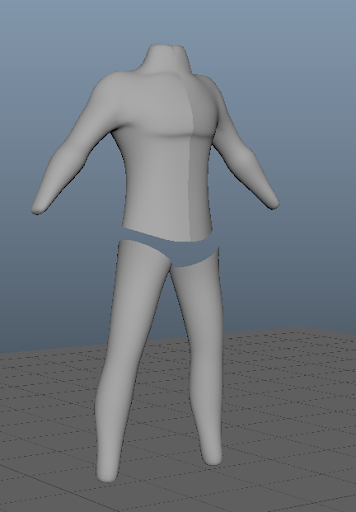
\includegraphics[width=5cm, height=5cm]
    {3D_model_body.png}}
  \end{figure}

  \begin{figure}[!htb]
    \center{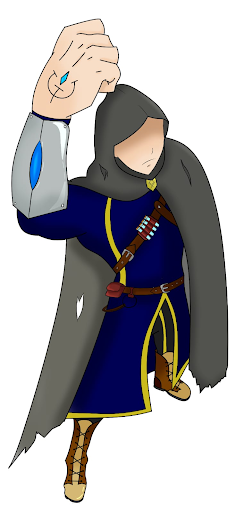
\includegraphics[width=5cm, height=5cm]
    {main_character_art_1.png}}
  \end{figure}

\newpage
 \subsection{Team Member Inclinations}
 \begin{description}
 \item Ayush - Animations, Player Scripting (Movement and interating with world)
 \item Luciano - Player Scripting (Abilities)
 \item Daniel - Player Scripting (Abilities)
 \item Christian - Asset Modelling, Import into Unity
 \item Samer - 
\end{description}

\end{document}